\documentclass[tikz,border=1pt]{standalone}
\usepackage{lmodern}\renewcommand{\familydefault}{\sfdefault}\usepackage[T1]{fontenc}
\usetikzlibrary{arrows.meta,positioning,calc}
\definecolor{ink}{HTML}{1A1A1A}\definecolor{gr}{HTML}{8A8A8A}\definecolor{grf}{HTML}{F2F2F2}
\definecolor{or}{HTML}{D55E00}\definecolor{orf}{HTML}{FDEEE6}\definecolor{gn}{HTML}{009E73}\definecolor{gnf}{HTML}{E6F5F0}
\definecolor{bl}{HTML}{0072B2}\definecolor{blf}{HTML}{E6F1F9}\definecolor{panel}{HTML}{FAFAFA}\definecolor{pline}{HTML}{C8C8C8}
\tikzset{
  box/.style={draw=gr,fill=grf,line width=0.6pt,rounded corners=2pt,minimum width=2.3cm,minimum height=0.9cm,text width=2.15cm,align=center,inner sep=2pt,font=\footnotesize,text=ink},
  mukv/.style={box,draw=or,fill=orf,line width=0.8pt},
  outc/.style={box,draw=gn,fill=gnf,line width=0.8pt},
  wide/.style={box,minimum width=4.6cm,text width=4.4cm,minimum height=0.8cm},
  wmukv/.style={wide,draw=or,fill=orf,line width=0.8pt,minimum height=1.05cm},
  half/.style={box,minimum width=2.0cm,text width=1.9cm,minimum height=1.05cm},
  hmukv/.style={half,draw=or,fill=orf,line width=0.8pt},
  hout/.style={half,draw=gn,fill=gnf,line width=0.8pt},
  hbox/.style={half,minimum height=0.8cm},
  data/.style={-{Stealth[length=4pt,width=3.5pt]},line width=0.6pt,ink},
  ctrl/.style={-{Stealth[length=4pt,width=3.5pt]},line width=0.6pt,or,dashed},
  ctrlg/.style={-{Stealth[length=4pt,width=3.5pt]},line width=0.6pt,gr,dashed},
  heat/.style={-{Stealth[length=4pt,width=3.5pt]},line width=0.7pt,gr,dotted},
  meas/.style={-{Stealth[length=4pt,width=3.5pt]},line width=0.6pt,gn,dash dot},
  kv/.style={-{Stealth[length=4pt,width=3.5pt]},line width=0.6pt,bl},
  lab/.style={font=\scriptsize,inner sep=1pt,text=ink},
  stepn/.style={circle,fill=or,text=white,font=\bfseries\tiny,inner sep=1pt,minimum size=9pt},
  head/.style={font=\bfseries\scriptsize,inner sep=1pt}
}
\newcommand{\bx}[2]{\textbf{#1}\\[-1pt]{\scriptsize #2}}
\begin{document}
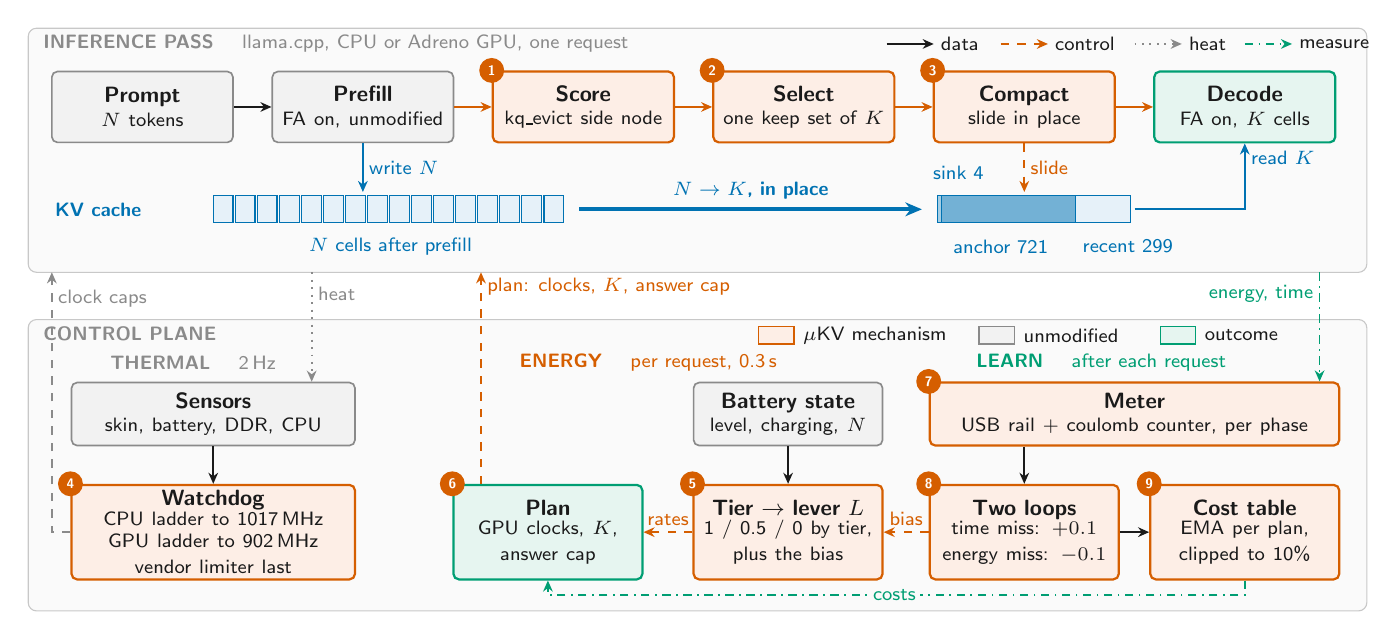
\begin{tikzpicture}[x=1cm,y=1cm]
% ================= panels =================
\fill[panel,draw=pline,rounded corners=3pt] (0,4.35) rectangle (17,7.45);
\fill[panel,draw=pline,rounded corners=3pt] (0,0.05) rectangle (17,3.75);
\node[head,anchor=north west,text=gr] at (0.15,7.4) {INFERENCE PASS \quad {\mdseries llama.cpp, CPU or Adreno GPU, one request}};
\node[head,anchor=north west,text=gr] at (0.15,3.7) {CONTROL PLANE};
% line-style legend on the top header line, swatch legend on the bottom header line
\draw[data] (10.9,7.25) -- (11.5,7.25);\node[lab,anchor=west] at (11.55,7.25) {data};
\draw[ctrl] (12.35,7.25) -- (12.95,7.25);\node[lab,anchor=west] at (13.0,7.25) {control};
\draw[heat] (14.05,7.25) -- (14.65,7.25);\node[lab,anchor=west] at (14.7,7.25) {heat};
\draw[meas] (15.45,7.25) -- (16.05,7.25);\node[lab,anchor=west] at (16.1,7.25) {measure};
\node[draw=or,fill=orf,minimum width=0.45cm,minimum height=0.22cm,inner sep=0] at (9.5,3.55) {};\node[lab,anchor=west] at (9.8,3.55) {$\mu$KV mechanism};
\node[draw=gr,fill=grf,minimum width=0.45cm,minimum height=0.22cm,inner sep=0] at (12.3,3.55) {};\node[lab,anchor=west] at (12.6,3.55) {unmodified};
\node[draw=gn,fill=gnf,minimum width=0.45cm,minimum height=0.22cm,inner sep=0] at (14.6,3.55) {};\node[lab,anchor=west] at (14.9,3.55) {outcome};
% ================= the pass =================
\node[box] (prompt) at (1.45,6.45) {\bx{Prompt}{$N$ tokens}};
\node[box] (prefill) at (4.25,6.45) {\bx{Prefill}{FA on, unmodified}};
\node[mukv] (score) at (7.05,6.45) {\bx{Score}{kq\_evict side node}};
\node[mukv] (select) at (9.85,6.45) {\bx{Select}{one keep set of $K$}};
\node[mukv] (compact) at (12.65,6.45) {\bx{Compact}{slide in place}};
\node[outc] (decode) at (15.45,6.45) {\bx{Decode}{FA on, $K$ cells}};
\draw[data] (prompt) -- (prefill);
\draw[data,or] (prefill) -- (score); \draw[data,or] (score) -- (select); \draw[data,or] (select) -- (compact); \draw[data,or] (compact) -- (decode);
\node[stepn] at (score.north west) {1};\node[stepn] at (select.north west) {2};\node[stepn] at (compact.north west) {3};
% KV strip
\node[lab,text=bl,font=\bfseries\scriptsize,anchor=west] at (0.3,5.15) {KV cache};
\foreach \i in {0,...,15}{\fill[blf,draw=bl,line width=0.4pt] (2.35+\i*0.28,4.98) rectangle (2.35+\i*0.28+0.25,5.32);}
\node[lab,text=bl] at (4.6,4.68) {$N$ cells after prefill};
\draw[kv] (prefill.south) -- (4.25,5.37) node[lab,text=bl,midway,right=1pt] {write $N$};
\draw[kv,line width=1.4pt,-{Stealth[length=6pt,width=5pt]}] (7.0,5.15) -- (11.35,5.15) node[lab,text=bl,font=\bfseries\scriptsize,midway,above=2pt] {$N \to K$, in place};
% compacted strip, proportional to the measured 4 / 721 / 299 split of K = 1024
\fill[bl!35!white,draw=bl,line width=0.4pt] (11.55,4.98) rectangle (11.60,5.32);
\fill[bl!55!white,draw=bl,line width=0.4pt] (11.60,4.98) rectangle (13.30,5.32);
\fill[blf,draw=bl,line width=0.4pt] (13.30,4.98) rectangle (14.00,5.32);
\node[lab,text=bl,anchor=west] at (11.45,5.62) {sink 4};
\node[lab,text=bl] at (12.35,4.68) {anchor 721};
\node[lab,text=bl,anchor=west] at (13.35,4.68) {recent 299};
\draw[ctrl] (compact.south) -- (12.65,5.37) node[lab,text=or,midway,right=1pt] {slide};
\draw[kv] (14.05,5.15) -- (15.45,5.15) -- (decode.south) node[lab,text=bl,pos=0.78,right=1pt] {read $K$};
% ================= control plane, two rows =================
\tikzset{colA/.style={box,minimum width=3.6cm,text width=3.4cm,minimum height=0.8cm},
         colA2/.style={colA,draw=or,fill=orf,line width=0.8pt,minimum height=1.2cm},
         colB/.style={box,minimum width=2.4cm,text width=2.25cm,minimum height=1.2cm},
         colB2/.style={colB,draw=or,fill=orf,line width=0.8pt},
         colBo/.style={colB,draw=gn,fill=gnf,line width=0.8pt},
         colBt/.style={box,minimum width=2.4cm,text width=2.25cm,minimum height=0.8cm},
         colC/.style={box,minimum width=5.2cm,text width=5.0cm,minimum height=0.8cm,draw=or,fill=orf,line width=0.8pt}}
\node[head,text=gr,anchor=west] at (1.0,3.2) {THERMAL \quad {\mdseries 2\,Hz}};
\node[head,text=or,anchor=west] at (6.2,3.2) {ENERGY \quad {\mdseries per request, 0.3\,s}};
\node[head,text=gn,anchor=west] at (12.0,3.2) {LEARN \quad {\mdseries after each request}};
\node[colA]  (sens)  at (2.35,2.55)  {\bx{Sensors}{skin, battery, DDR, CPU}};
\node[colA2] (wd)    at (2.35,1.05)  {\bx{Watchdog}{CPU ladder to 1017\,MHz\\ GPU ladder to 902\,MHz\\ vendor limiter last}};
\node[colBt] (batt)  at (9.65,2.55)  {\bx{Battery state}{level, charging, $N$}};
\node[colBo] (plan)  at (6.6,1.05)   {\bx{Plan}{GPU clocks, $K$,\\ answer cap}};
\node[colB2] (lever) at (9.65,1.05)  {\bx{Tier $\to$ lever $L$}{1 / 0.5 / 0 by tier,\\ plus the bias}};
\node[colC]  (meter) at (14.05,2.55) {\bx{Meter}{USB rail + coulomb counter, per phase}};
\node[colB2] (loops) at (12.65,1.05) {\bx{Two loops}{time miss: $+0.1$\\ energy miss: $-0.1$}};
\node[colB2] (table) at (15.45,1.05) {\bx{Cost table}{EMA per plan,\\ clipped to 10\%}};
\node[stepn] at (wd.north west) {4};\node[stepn] at (lever.north west) {5};\node[stepn] at (plan.north west) {6};
\node[stepn] at (meter.north west) {7};\node[stepn] at (loops.north west) {8};\node[stepn] at (table.north west) {9};
\draw[data] (sens) -- (wd);
\draw[data] (batt) -- (lever);
\draw[ctrl] (lever) -- (plan) node[lab,text=or,midway,above=1pt] {rates};
\draw[data] (meter.south -| loops) -- (loops.north);
\draw[data] (loops) -- (table);
\draw[ctrl] (loops.west) -- (lever.east) node[lab,text=or,midway,above=1pt] {bias};
\draw[meas] (table.south) -- (15.45,0.25) -- (6.6,0.25) -- (plan.south);
\node[lab,text=gn,fill=panel,inner sep=1.5pt] at (11.0,0.25) {costs};
% ================= links between the panels =================
\draw[ctrlg] (wd.west) -- (0.3,1.05) -- (0.3,4.35) node[lab,text=gr,pos=0.9,right=1pt] {clock caps};
\draw[heat] (3.6,4.35) -- (sens.north -| 3.6,0) node[lab,text=gr,pos=0.2,right=1pt] {heat};
\draw[ctrl] (plan.north -| 5.75,0) -- (5.75,4.35) node[lab,text=or,pos=0.93,right=1pt] {plan: clocks, $K$, answer cap};
\draw[meas] (16.4,4.35) -- (meter.north -| 16.4,0) node[lab,text=gn,pos=0.2,left=1pt] {energy, time};
\end{tikzpicture}
\end{document}
